\documentclass[12pt]{article}

\usepackage{cls}
\usepackage{tipa}
\usepackage{enumerate}
\usepackage{float}
\title{The co-fronting of the tense back vowels\\ in York, northern England}
\author{Daniel Lawrence}
\organization{The University of Edinburgh}

\begin{document}

\maketitle

\section{Introduction}

Research into vocalic changes of the past century has yielded a set of strong generalizations which appear to apply across varieties of English. One such pattern is the tendency for historically back vowels to move to the front of the vowel space -- Labov's (1994) `Principle III' of vowel shifts. Where back vowel fronting is attested, it appears to exhibit a number of recurrent patterns in terms of a) the relationship between consonant-on-vowel coarticulation and diachronic fronting, b) the relative timing and speed of change in the vowels affected, and c) the phonetic relationship between the categories undergoing change. The fact that these processes exhibit such striking similarities across dialects implies that they may reflect some underlying constraints on the organization of vowel systems and the ways in which those systems may change. The present paper extends research in this area by presenting evidence of the fronting of the tense back vowels \textipa{/o/} and \textipa{/u/} in a variety of northern British English, with a view to testing whether previous generalizations regarding these changes apply in this community. 

\subsection{Previous work on \textipa{/u/} and \textipa{/o/} fronting}

The fronting of \textipa{/o/} and \textipa{/u/}  has been documented extensively across the United States (e.g. Labov et al. 2006, Baranowski 2008; Hall-Lew 2009), Australia (Cox 1999) and New Zealand (Easton \& Bauer 2000), as well as in varieties of British English (Jansen 2010, Kerswill \& Williams 2000 Watt \& Tillotson 2001). In addition to being an extremely common pattern of change, the fronting of back vowels seems to possess a number of recurrent properties. The following four generalizations will be the focus of the present work:

\begin{enumerate}
\item{Back vowel fronting has its primary source in patterns of coarticulatory variation, the effects of which decrease over time.}
\item{\textipa{/o/} fronting occurs only in dialects which also front \textipa{/u/}.}
\item{Where both vowels undergo fronting, \textipa{/u/} fronting precedes \textipa{/o/} fronting temporally, and \textipa{\textipa{/o/}} tends to change more slowly than \textipa{\textipa{/u/}}.}
\item{In varieties where both vowels undergo fronting, the nucleus of \textipa{\textipa{/u/}} remains more advanced in F2 space than that of \textipa{\textipa{/o/}}.}
\end{enumerate}

The first of these generalizations refers to the fact that back vowels, especially \textipa{/u/}, are often fronted in post-alveolar contexts as a consequence of consonant-on-vowel coarticulation. Change in these vowels tends to involve productions in non-fronting contexts gradually moving forward, while productions in conditioning environments remain relatively constant. This pattern, reported in e.g. Durian, (2012); Harrington et al. (2006) and Hall-Lew (2011), can be taken as evidence of an internal pressure in favour of back-vowel fronting, perhaps due to learners' reanalysis of fronted allophones as production targets (e.g. Ohala 1994; Harrington et al. 2006) and/or the articulatory cost of maintaining a category with widely separated contextual variants (Harrington et al. 2011). Regardless of the psychological or physiological explanation of this pattern, its prevalance implies that coarticulatory processes provide a reasonable source for diachronic fronting, meaning that the cross-varietal prevalence of this change is not necessarily the product of geographical diffusion, as has sometimes been implied.

The second generalization is demonstrated very clearly in Labov et al. (2005).   Surveying the relationship between \textipa{/o/} and \textipa{/u/} fronting across dialects, they demonstrate that North American varieties of English can be divided into three groups -- those that front neither \textipa{/u/} nor \textipa{/o/}, those that front \textipa{/u/} alone, and those that front both \textipa{/u/} and \textipa{/o/}. In no cases do they find a variety where \textipa{/o/} fronts in the absence of the fronting of \textipa{/u/}. This observation has also been used to motivate arguments regarding the temporal relationship between change in the two vowels (generalization 3 above) -- in Labov's (1994) model of chain-shifting, \textipa{/u/} fronting is said to occur prior to \textipa{/o/} fronting, triggering the raising of the latter to the position of the former. Furthermore, Labov (1994) observes that \textipa{/u/} tends to remain more advanced in the vowel space than \textipa{/o/} when both vowels undergo fronting. 

While these facts are well-attested for North American dialects, and to some extent in RP (Harrington, 2007, Harrington et al. 2008), there is some debate as to whether northern dialects of British English are exceptional with regard to these patterns. For example, it has been claimed that \textipa{\textipa{/o/}} fronting occurs in the absence of \textipa{\textipa{/u/}} fronting in Bradford, West Yorkshire (Watt \& Tillotson 2001), as well as in Newcastle (Watt 2000). Haddican et al.`s (2013) study of York speech, which provides the impetus for the present work, suggests that northern British varieties may partially contradict previous generalizations due to the social indexing of dynamic vowel variation in the UK. The variable diphthongization of \text{\textipa{/o/}} is widely cited as a key shibboleth of northern/southern regional identity in Britain (e.g. Watt 2000). It is thus reasonable to expect, as Haddican et al. (2013) claim, that patterns of resistance to an otherwise extremely regular pattern of vowel shift might be observed in northern England, reflecting the social values associated with dynamic characteristics of the competing forms.

\section{Data \& Methods}

\subsection{Data}

Data are taken from a corpus of recordings collected from 52 individuals born between 1935 and 2000. Speakers were recruited using convenience sampling, as is typical in variationist sociolinguistic work. Table 1 provides the basic demographic information of the sample, including participatns' gender and year of birth (collected from a post-interview questionnaire), and their grouping according to a \textit{mobility index}. This index was one of three factors derived from informants' responses to the interview questions (see section 2.3).

\vspace*{6pt}
\begin{table}[htbp]
\centering
\begin{tabular}{l|l|l|l|l}
Mobility index&\multicolumn{2}{l|}{Upper}&\multicolumn{2}{l}{Lower}\\
\hline
Gender& Female& Male & Female & Male\\
\hline
1935-1960 & 6&4&2&2\\
 1961-1980& 2 &0&3&4\\
1981-2000&  7&3&10&4\\

\end{tabular}
\caption{Characteristics of the speaker sample}
\end{table}
\vspace*{6pt}

The data include a) a 100-item wordlist, including 15 tokens of each vowel in a range of phonetic environments plus fillers; b) a map task (Anderson et al., 1991) using a selection of words from the word list and c) a sociolinguistic interview, including a range of questions relevant to the speakers' social background and identity with regard to York and the north of England. 

\subsection{Measurement}

Vowels were segmented from the first to the last glottal pulse visible in the spectrogram, and measurements of F1, F2 and F3 were taken at 20 equidistant points along the vowel trajectory. The present analysis will focus on F2 trajectories, which provide a relatively reliable reflection of the degree of fronting and diphthongization for these vowels. Measurements were normalized using the centroid method of Watt \& Fabricius (2002), using the mean midpoint values of each speakers' \textipa{/A/} and \textipa{/i/} productions as centroids. The formant values provided in the present analyses are of the form $F^n/S (F^n)$, i.e. the ratio of the measured frequency in Hz to the centroid frequency of that formant for the speaker being analyzed.

\subsection{Statistical analysis}

The results presented in the following sections use the statistical technique of \textit{Generalized Additive Modeling}, which allow vowel tokens to be summarized as smooth functions of time. Winter \& Wieling (2016) give a concise summary of the application of such models to time-varying linguistic data. The relevance of such models to the present study is that they allow the analysis to capture non-linear changes in the dynamic properties of vowels, without enforcing any a priori assumptions about the shape of formant trajectories and trajectory of change. The models presented in this paper predict normalized F2 as a function of time, plus the variables listed below:

\vspace*{6pt}
\begin{table}[H]
\centering
\begin{tabular}{l|l}
Variable&Form \\
\hline
Phonetic environment & \textipa{/u/}: Tuw Juw Kuw uwL uw\\&\textipa{/o/}: Tow Kow ow owN owL\\
Log duration& Continuous \\
Speaker year of birth& Continuous (1935-2000)\\
Speaker gender& M/F \\
General SES index & (Higher/Lower) \\
Speaker local identity index & (Higher/Lower) \\
Speaker mobility index & (Higher/Lower) \\
\end{tabular}
\caption{Variables tested}
\end{table}
\vspace*{6pt}

The phonetic environments coded represent three places of articulation of the preceding consonant -- post-coronal contexts excluding nasals and \textipa{/j/} (\textit{Tuw/Tow}), post-velar contexts excluding nasals (\textit{Kuw/Kow}) and all other contexts (\textit{ow/uw}). For \textipa{/u/}, Seperate codes were included for preceding /j/, known to heavily favour fronting (\textit{Juw}), and following \textipa{/l/}, known to heavily inhibit it (\textit{uwL}). Similarly, seperate categories were coded for \textipa{/o/} tokens followed by a nasal (\textit{owN}), and those followed by \textipa{/l/} (\textit{owL}).

\vspace*{6pt}
\begin{table}[!htbp]
\centering
\begin{tabular}{l|l|l}
Vowel&Variant&Criteria \\
\hline
\textipa{/u/}&Tuw & Preceding \textipa{/j/}\\
&Tuw & Preceding coronal\\
&Kuw & Preceding velar\\
&uwL & Following \textipa{/l/}\\
&uw & All other contexts \\
\textipa{/o/}&Tow & Preceding coronal\\
&Kow & Preceding velar\\
&Kow & Following \textipa{/l/}\\
&Kow & Following nasal\\
&ow & All other contexts
\end{tabular}
\caption{Coding criteria}
\end{table}
\vspace*{6pt}

In addition to the speakers' age and gender, which were collected through a questionnaire, three social indices were created based on a set of questions asked during the sociolinguistic interview. Three underlying dimensions were derived from an exploratory factor analysis of these responses -- a general SES index, a local identity index, and a mobility index; for brevity, the specific details of this factor analysis will be left for a future version of this work. The general SES index, which groups together a measure of the speaker's level of education and employment status. The local identity index measures the degree to which each individual identifies as someone from York and the extent to which they are invested in the local community. The mobility index groups together a set of characteristics related to geographical and social mobility, e.g. whether or not the speaker travels regularly within the UK; whether or not they have worked and studied in York for an extended period, and whether or not they plan to stay in York permanently.

 The baseline models included constant terms for linguistic factors and their smooth interactions with the phonetic environment. Random smooths were included for each speaker, allowing the model to account for individual variation in vowel production. Model selection was performed by stepping up from the minimal models, retaining variables which significantly improved the model fit according to a Chi-Square test on the difference in fREML scores. Table 4 describes the predictors identified as significant for each vowel (p$<$0.001 in all cases).
\vspace*{6pt}
\begin{table}[H]
\centering
\begin{tabular}{l|l}
Vowel&Variables selected\\
\hline
\textipa{/u/}&Phonetic environment\\
&Log duration\\
&Speaker year of birth\\
&Speaker year of birth : phonetic environment\\
\textipa{/o/}&Phonetic environment\\
&Log duration\\
&Speaker year of birth\\
&Speaker year of birth : phonetic environment\\
&Mobility index\\
&Speaker year of birth : mobility index
\end{tabular}
\caption{Variables selected as significant for each vowel}
\end{table}
\vspace*{6pt}

For both vowels, speaker year of birth was selected as significant, indicating evidence of apparent-time change in both vowels. This will be explored in section 3.1. The significant interaction between phonetic environment and year of birth implies that the change is more vigorous in some phonetic environments than others; this will be discussed in section 3.2. Interestingly, the only additional non-linguistic factor selected was the mobility index for \textipa{/o/}; the interaction between this index and year of birth suggests that speakers' contact with external varieties may constrain change in this vowel, which will be discussed in section 5. The remainder of this paper will describe these effects in more detail and relate them to the four generalizations outlined in the introduction.

\section{Results}
\subsection{Evidence of \textipa{\textipa{/o/}} and \textipa{\textipa{/u/}} fronting in York}
Figure 1 visualizes the main effect of speaker year of birth on the second formant of \textipa{\textipa{/o/}} and \textipa{\textipa{/u/}}, plotted at the 10th measurement point. The results demonstrate that the F2 midpoint of both vowels is reliably higher with increasing speaker year of birth, providing apparent-time evidence that both vowels have undergone fronting over the past $~$65 years. Change in \textipa{\textipa{/u/}} appears to have proceeded in a slightly more regular fashion that change in \textipa{\textipa{/o/}}, evidenced in the slightly tighter clustering of speaker means around the model predictions in Figure 1.  Also noteworthy is that change in \textipa{\textipa{/u/}} appears to have been much more radical than change in \textipa{\textipa{/o/}}, with change in \textipa{\textipa{/u/}} resulting in an increase of around .5 normalized units versus around .2 in \textipa{\textipa{/o/}}. 

\vspace*{6pt}
\begin{figure}[H]
\centering
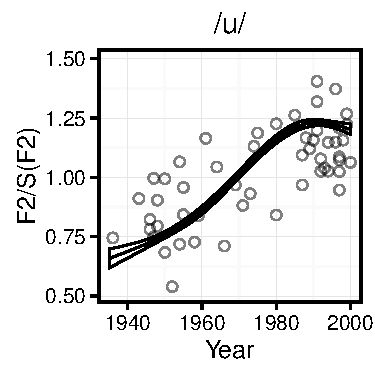
\includegraphics{uwchange}
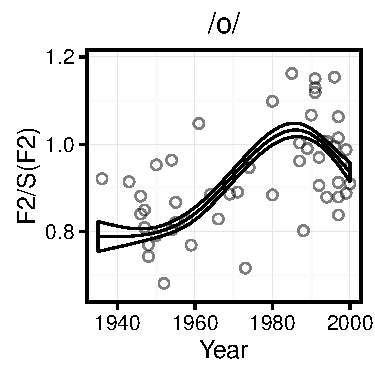
\includegraphics{owchange}
\caption{Evidence of \textipa{\textipa{/o/}} and \textipa{\textipa{/u/}} fronting}
\end{figure}
\vspace*{6pt}

\subsection{The coarticulatory basis of \textipa{\textipa{/u/}} and \textipa{\textipa{/o/}} fronting}

The first generalization to be tested regards the proposal that coarticulatory variation provides the primary source for back vowel fronting. Under this proposal, it would be expected that the oldest speakers in the sample would demonstrate a wide range of variation in \textipa{/u/} and \textipa{/o/} conditioned by phonetic environment. Change would be expected to be most vigorous in those forms \textit{least} subject to coarticulatory fronting, with little or no change predicted for the \textit{most} conditioning environments. As a result, the effect of coarticulatory variation would be predicted to decrease with speaker year of birth, reflecting the generalization of the fronted targets across environments. 

\vspace*{6pt}
\begin{figure}[H]
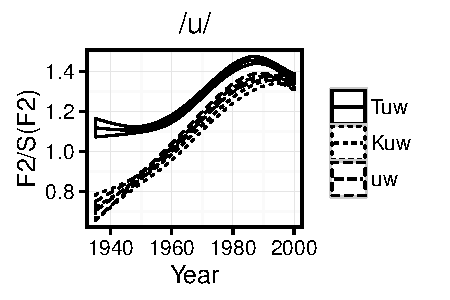
\includegraphics{uwphoneticconditioning}
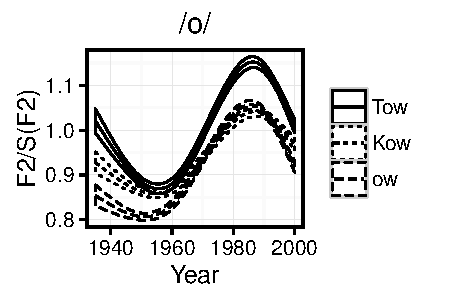
\includegraphics{owphoneticconditioning}
\caption{Changes in the phonetic conditioning of \textipa{/o/} and \textipa{/u/} fronting.}
\end{figure}
\vspace*{6pt}


Figure 2 demonstrates the role of coarticulation in conditioning back vowel fronting in this variety, plotting the significant interaction of speaker year of birth and phonetic environment for the \textit{Tuw/Tow}, \textit{Kuw/Kow} and \textit{uw/ow} contexts. Both vowels show some evidence of a reduction of coarticulatory effects over time, although this pattern is most noticeable for \textipa{/u/}. For the oldest speakers in the sample, \textipa{/u/} is produced with a phonetically fronted variant following a coronal consonant (e.g. in \textit{two}), and has a back variant in all other contexts. The change takes place primarily in the non-phonetically fronting contexts, meaning that the youngest speakers in the sample produce forms such as \textit{food} and \textit{noon} with the fronted variant which was previously restricted to postcoronal environments. This pattern is less clear in the case of \textipa{/o/}. Although there appears to be a weaker distinction between Kow and ow contexts among speakers born after \textasciitilde1960, there is no evidence of the rapid re-alignment of allophones seen in \textipa{/u/} fronting. Taken together, these results suggest that back vowel fronting in York adheres to the first generalization discussed in the introduction of this paper, at least in the case of \textipa{/u/}. As has been reported in other varieties of English, the coarticulatory fronting of the back vowels appears to provide a source for diachronic change. The clearest evidence for this comes from change in \textipa{/u/}, where the contexts demonstrating the strongest coarticulatory bias toward fronting show a smaller and less vigorous change in comparison to contexts which have no such bias. 

\subsection{The relationship between \textipa{/u/} and \textipa{/o/}}
The second generalization to be discussed regards the cross-dialectal relationship between \textipa{/o/} and \textipa{/u/}. The fact that both \textipa{/u/} and \textipa{/o/} appear to have undergone fronting confirms that this variety is not exceptional with regard to the generalization that \textipa{/o/} fronting tends occur only in varieties which also front \textipa{/u/}. Examining estimates of the relative timing of change in the two vowels sheds further light on this relationship, and speaks to the third generalization discussed in the introduction. Figure 3 visualizes the estimated trajectories of change for both vowels (left-hand panel), and the estimated rate of change in F2 (right hand panel), generated by differentiating the curves in the left-hand panel. The vertical line represents an estimate of the point at which \textipa{/o/} began to front.

\vspace*{6pt}
\begin{figure}[H]
\centering
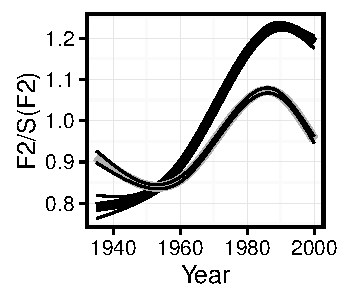
\includegraphics{owuwparallel.pdf}
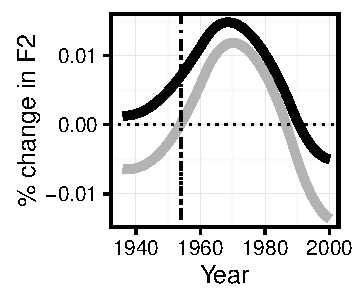
\includegraphics{owuwparallelROC.pdf}
\caption{The temporal relationship of \textipa{/o/} and \textipa{/u/} fronting.}
\end{figure}
\vspace*{6pt}

While our faith in these estimates should be balanced against the relatively small size of the present sample, a number of observations can be made. Firstly, there is clear evidence that change in \textipa{/u/} began before change in \textipa{/o/}; in fact, there appears to have been a lag of around 20 years between the onset of change in the two vowels. \textipa{/u/} fronting was already in progress for speakers born in 1940, while change in \textipa{/o/} began in the speech of those born around the mid 1950s, visible where the \textipa{/o/} curve crosses zero in the right-hand panel. Consistent with previous findings, the rate of fronting for \textipa{/o/} remains lower than that of \textipa{/u/} throughout the change. A second observation involves the relative position of the two vowels in F2 space, and its relationship with the timing of change in \textipa{/o/}. Note that, for speakers born around 1940, the nucleus of \textipa{/o/} is typically in advance of that of \textipa{/u/}. As \textipa{/u/} begins to front, its F2 target begins to approach that of \textipa{/o/}, and the point at which \textipa{/o/} fronting begins is roughly the same point at which the two vowels are parallel in F2 space (\textasciitilde1954, marked with a vertical dotted line). From that point on, while both \textipa{/u/} and \textipa{/o/} undergo fronting, the relative position of the two vowels appears to be preserved, such that the nucleus of \textipa{/u/} remains reliably retracted in relation to \textipa{/o/}. The robustness of this pattern is demonstrated in Figure 4, which visualizes each speakers' mean \textipa{/u/} and \textipa{/o/}  nuclei as a function of their year of birth.

\vspace*{6pt}
\begin{figure}[H]
\centering
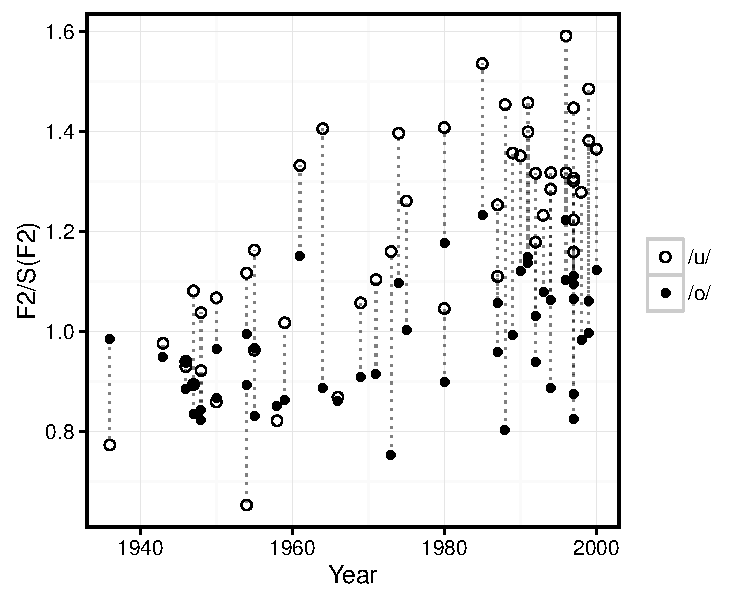
\includegraphics[scale=.9]{resistance1.pdf}
\caption{Relationship between \textipa{/o/} and \textipa{/u/} fronting over time.}
\end{figure}
\vspace*{6pt}

Among speakers born before 1954 (to the left of the dotted line), some individuals produce \textipa{/u/} further back than \textipa{/o/}, and others produce \textipa{/o/} further back than \textipa{/u/}. However, after the actuation of change in \textipa{/o/}, each individual has a \textipa{/u/} nucleus reliably in advance of that of \textipa{/o/}. This observation relates to the fourth generalization mentioned in the introduction, namely that \textipa{/u/} tends to be further forward in F2 space than \textipa{/o/} varieties which front both vowels. What is striking about the present results is that they indicate that this may not have been true before the actuation of \textipa{/o/} fronting, but for speakers born after that point, a near-exceptionless relationship between the two vowels emerges.

Further evidence of the relationship between \textipa{/o/} and \textipa{/u/} fronting is demonstrated in Figure 5, which plots the within-speaker relationship between the nuclei of the two vowels.

\vspace*{6pt}
\begin{figure}[H]
\centering
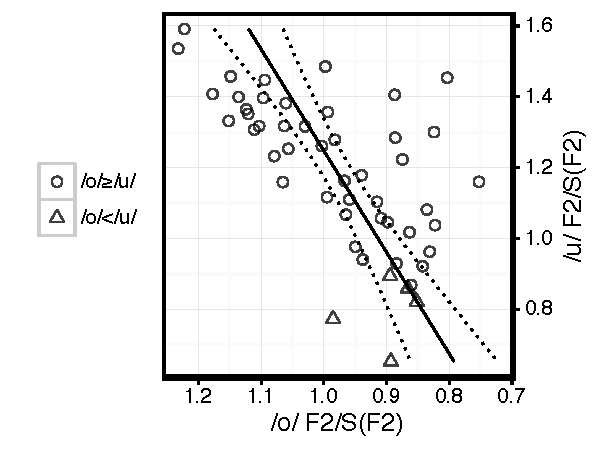
\includegraphics{owuwcorrelation.pdf}
\caption{Within-speaker relationship between \textipa{/o/} and \textipa{/u/}.}
\end{figure}
\vspace*{6pt}

Figure 5 provides a further observation of relevance, this time with regard to the claim that \textipa{/o/} fronting only occurs in varieties which also front \textipa{/u/}. Considering the within-speaker relationship between the two vowels reveals that the cross-dialectal pattern is not only true when comparing dialects, but also when comparing individuals within a single variety.  While there is a clear correlation between an individuals' degree of \textipa{/o/} fronting and their degree of \textipa{/u/} fronting, this correlation is driven by the lack of data points in the bottom-right hand corner of the plot. While a number of speakers retain back \textipa{/o/} and back \textipa{/u/} (bottom, right-hand corner); some front only \textipa{/u/} (top, right-hand corner), and some front both \textipa{/o/} and \textipa{/u/} (top, left-hand corner), few, if any speakers front \textipa{/o/} without participating in \textipa{/u/} fronting. This is exactly the same pattern reported cross-dialectally, here robustly replicated within a single community. This provides convincing evidence that the phonetic relationship between \textipa{/o/} and \textipa{/u/} does not simply reflect historical accident -- rather, it implies that the forward drift of \textipa{/u/} may have been the \textit{triggering event} (Labov 2008) for change in \textipa{/o/}. The fact that change in \textipa{/o/} appears to have started roughly as \textipa{/u/} advanced past it further supports this claim.

\section{The internal motivation for \textipa{/o/} and \textipa{/u/} fronting}
To summarize the findings presented so far, the data provide robust evidence of the fronting of \textipa{/o/} and \textipa{/u/} over the past 65 years in York speech. Change in these vowels is consistent with previous accounts of similar developments across varieties of English in a number of ways:

\begin{itemize}
\item{The source of diachronic \textipa{/u/} fronting appears to be related to synchronic consonant-on-vowel coarticulation, the effects of which decrease over time; however, this may be less true for \textipa{/o/}.}

\item{\textipa{/u/} fronting proceeds \textipa{/o/} fronting temporally, with a lag of $~$20 years.}

\item{A speakers' participation in \textipa{/o/} fronting is conditional on their participation in \textipa{/u/} fronting -- no speaker fronts \textipa{/o/} without also fronting \textipa{/u/}.}

\item{There appears to be a robust pressure to maintain a relationship between the nuclei of \textipa{/o/} and \textipa{/u/}, such that the vast majority of speakers' produce \textipa{/o/} with a more retracted nucleus than \textipa{/u/}.}
\end{itemize}

These facts permit a tentative account of the way change in the tense back vowels of this variety progressed over the past 65 years. At the beginning of the change there was a state where \textipa{/u/} was the most back category in the system, and was subject to a pattern of coarticulation whereby it was strongly fronted in post-coronal contexts. During this state, the nucleus of \textipa{/o/} was relatively more centralized that that of \textipa{/u/}. The fronting of \textipa{/u/} then began to take place, with non-post-coronal allophones gradually shifting forward to meet the phonetically fronted post-coronal realizations. This fronting of \textipa{/u/} triggered the fronting of \textipa{/o/}, which began at roughly the same time that the nucleus of \textipa{/u/} advanced further forward than that of \textipa{/o/}. At this point, \textipa{/o/} was reanalyzed as the most back category, leading to the observed tendency for speakers to maintain an \textipa{/u/} nucleus in advance of \textipa{/o/}.

\section{Resistance to phonetic change}

The trajectory of change thus far described has an interesting consequence. For a speaker born directly after the reanalysis of \textipa{/o/} as the most back category, it would seem that the realizational possibilities of \textipa{/o/} are limited, given that that speaker would presumably also have a relatively back realization of \textipa{/u/}, and thus be under pressure to maintain a back \textipa{/o/} variant. However, as change in \textipa{\textipa{/u/}} progresses, the realizational possibilities for \textipa{\textipa{/o/}} increase -- a speaker may retain a very back form or front \textipa{\textipa{/o/}} to the same extent that they front \textipa{\textipa{/u/}}. While some speakers participate in both \textipa{\textipa{/u/}} and \textipa{\textipa{/o/}} fronting, others appear to resist fronting \textipa{\textipa{/o/}}. This can be verified in Figure 4 (p.8) -- speakers born before 1954 have relatively little distance between the two vowels; after the onset of \textipa{/o/} fronting, while all speakers keep \textipa{\textipa{/u/}} in front of \textipa{\textipa{/o/}}, some appear to retain a back \textipa{\textipa{/o/}} variant, equally or even more back than the oldest speakers in this sample. This pattern is summarized below, ignoring for a moment the possible role of diphthongization:

\vspace*{6pt}
\begin{table}[H]
\begin{exe}
\ex
\centering
\setlength{\tabcolsep}{0.5cm}
\label{haddican-results}
\begin{tabular}{lllll}
&i.&ii.&iii.&\\
/u/ &  u  & \textipa{0} &\textipa{y}&\\
/o/ &  o  & o &\textipa{o}\textasciitilde\textipa{8}&\\
\end{tabular}
\end{exe}
\end{table}
\vspace*{6pt}
At the earliest state of the change, both vowels are back (i); \textipa{/u/} then begins to front (ii.), exerting a pressure upon \textipa{/o/} to also move forward (iii.). At the end of the change, \textipa{/u/} fronting moves to completion across the community, while some speakers retain a relatively back \textipa{/o/} variants. What causes this resistance to fronting among certain younger speakers? Given that the variable diphthongization of \textipa{\textipa{/o/}} is widely noted as a marker of regional identity, it is reasonable to predict that dynamic properties of this vowel might play a role. Exploring the relationship between fronting and diphthongization reveals an interesting pattern, demonstrated in Figure 6, which plots each speaker's normalized mean F2 at the midpoint against their mean trajectory length, measured as the Euclidean distance between the 5th and 15th measurement points in F1-F2 space. The three convex hulls represent the output of a density-based clustering technique (Ester et. al 1996), which attempts to group the datapoints into spatially-related clusters. The clusters of speakers identified represent three groups in acoustic space: some have a back, monophthongal \textipa{\textipa{/o/}}; some have back, diphthongal \textipa{\textipa{/o/}}, and some have a fronted, diphthongal variant. Notably, there seems to be a lack of cases of fronted, monophthongal \textipa{\textipa{/o/}}. The speakers who were shown to resist fronting in Figure 5 are those who retain a monophthongal variant. The relationship between this pattern and age is also of interest -- while older (`O') speakers demonstrate a more-or-less continuous distribution on the Euclidean distance (vertical) dimension, middle (`M') and younger (`Y') speakers appear to `sort' themselves into one of two groups -- either adopting the very fronted diphthong, or retaining a relatively back monophthong. In other words, it seems that subgroups of this community have become more distinct over time in terms of their \textipa{/o/} productions.

\vspace*{6pt}
\begin{figure}[H]
\centering
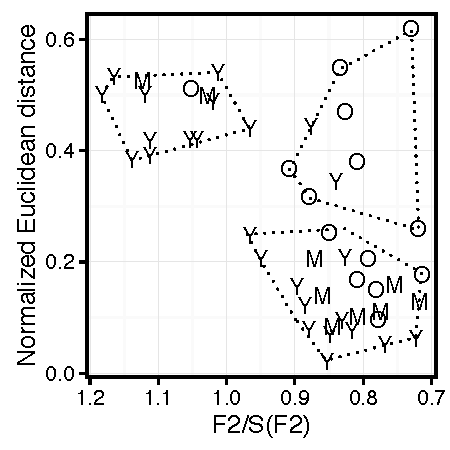
\includegraphics[scale=0.85]{ofrontingdip.pdf}
\caption{Relationship between \textipa{/o/} fronting and diphthongization.}
\end{figure}
\vspace*{6pt}

These data allow further detail to be added to the schematization of this change, now taking the role of diphthongization into account:

\vspace*{6pt}

\begin{table}[H]
\begin{exe}
\ex
\centering
\setlength{\tabcolsep}{0.5cm}
\label{haddican-results}
\begin{tabular}{llllll}
&i.&ii.&iii.&&\\    
/u/ &  \textipa{u} &  \textipa{0} &  \textipa{y} & \textipa{y} \\
/o/ &    o $\sim$ \textipa{oU} &  o $\sim$ \textipa{oU}        &  o       &  \textipa{\textschwa U}      
\end{tabular}
\end{exe}
\end{table}
\vspace*{6pt}

The general pattern appears to involve the amplification of differences between monophthongal and diphthongal speakers, who now differ from each other not only in terms of diphthongization, but also fronting. The apparent lack of fronted monophthongal \textipa{/o/} is consistent with Haddican et al.'s (2013) recent findings on this community, with the exception that the authors found fronted monophthongs among their middle age group (speakers born 1967-1981), in contrast to the complete absence of such forms in the present data. There are at least two possible explanations for a pattern like this. \begin{enumerate}[(i)]\item{Monophthongal speakers may have resisted the internal pressure to front \textipa{/o/}, leading to them lagging behind diphthongal speakers.}
\item{Diphthongal speakers may have accelerated the internal pressure to front \textipa{/o/} fronting further, leading to their more advanced realizations.}
\end{enumerate}

With regard to the first explanation, if we imagine a general pressure to front both \textipa{\textipa{/o/}} and \text{\textipa{/u/}}, then it might be proposed that speakers avoid participating in \textipa{\textipa{/o/}} fronting due to a stigmatization of fronted, monophthongal variants. This is similar to the phenomenon of \textit{sound change supression} mentioned in Kroch (1978) and Thomason (2016), in which the stigmatization of certain sounds leads to their loss from a particular variety. Haddican et al. (2013) develop this argument in detail, proposing that younger speakers associate monophthongal \textipa{/o/} with a stigmatized, class-based stereotype, the \textit{chav}. Under this account, all speakers are subject to an internally-motivated pressure to front, but this pressure is blocked by the negative social indexing among monophthongal speakers.

A second explanation can also be entertained -- rather than this being a pattern of resistance per se, it could be that fronting is accelerated among diphthongal speakers, either due to social factors, the temporal-dynamic characteristics of their \textipa{\textipa{/o/}} productions (i.e. diphthongs tend to be more fronted anyway), or some combination of the two.

 Exploring the patterning of dynamic variation of \textipa{\textipa{/o/}} across speaker groups strongly suggests that this explanation is better supported by the data. Figure 7 plots predicted contours for the high-mobility and low-mobility groups, faceted by year of birth.


\vspace*{6pt}
\begin{figure}[H]
\centering
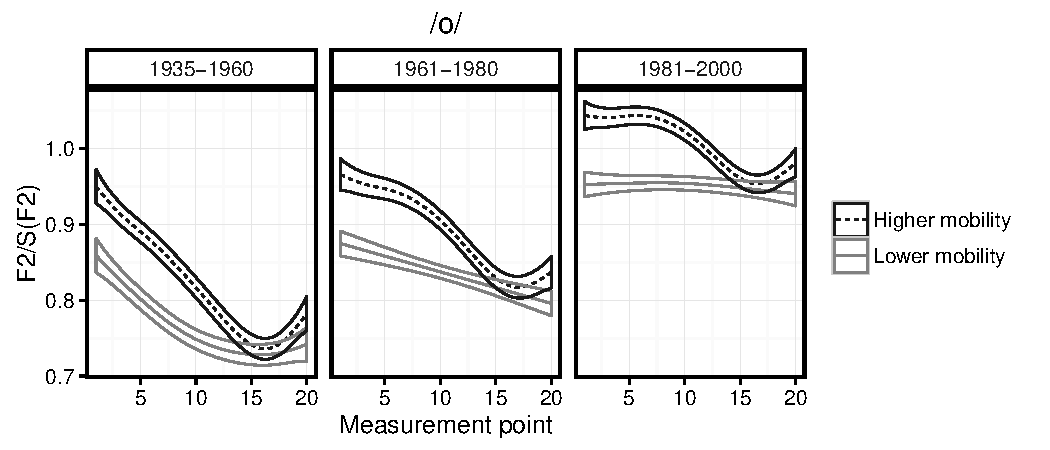
\includegraphics[scale=0.9]{owdynamicsclass.pdf}
\caption{Estimated \textipa{/o/} F2 trajectory by decade and mobility group.}
\end{figure}
\vspace*{6pt}
 It is clear that for all age groups, more mobile speakers are reliably more diphthongal than less mobile speakers, presumably representing the more mobile speakers appoximating a Southern Standard British English form. While Figure 6 seemed to imply that fronting was heavily inhibited among monophthongal speakers, the trajectory models imply that some degree of fronting does actually take place, albeit less dramatic than in the case of diphthongal speakers. Fronting appears to have two effects -- fronting among less mobile speakers involves a shift across the entire F2 trajectory, as well as fronting at the offglide. This results in an overall more monophthongal average trajectory among younger, less mobile speakers. Among more mobile speakers, fronting happens at both the vowel onset (around the seventh measurement point) and offglide, resulting in a much more curved trajectory among younger speakers. A side effect of this interaction between fronting and diphthongization is that fronting appears more advanced among the more mobile group. Overall, this suggests that the observed pattern of `resistance' may not be resistance at all, but rather an example of contact-related factors facilitating an internal bias. It seems that fronting may have lead the amplification of existing socially-conditioned differences in the temporal dynamics of the back vowels, leading to more mobile speakers producing more fronted, diphthongal realizations than less mobile speakers. While the account of social-indexically motivated resistance presented in Haddican et al. (2013) is perfectly feasible, paying attention to the fine-grained temporal details of this vowel suggests that an explanation based on the combined effects of speaker mobility and internal pressures better fit the data.

\section{Conclusion}

This paper has presented apparent-time evidence of the fronting of the back upgliding vowels over the past \textasciitilde65 years in York, northern England. Its core aim was to test a set of cross-varietal generalizations regarding back vowel fronting, including the relationship between back vowel fronting and consonant-on-vowel coarticulation, the relative timing of parallel back vowel shifts, and the phonetic relationship between the categories undergoing change. In general, the findings suggest that back vowel fronting in York conforms to previous generalizations, adding to the evidence that Labov's `Principle III' of vowel shifting may apply across varieties of English, and possibly reflect some general biases toward certain kinds of change cross-linguistically. 

This investigation has revealed a number of innovative findings. Firstly, not only did change in \textipa{/o/} begin after change in \textipa{/u/} in this variety, it initiated at roughly the point where the nucleus of \textipa{\textipa{/u/}} passed that of \textipa{\textipa{/o/}} in F2 space. This lead to speakers adopting an almost exceptionless constraint on the relative position of the two vowels, with each individual's \textipa{\textipa{/u/}} nucleus remaining reliably fronter than that of \textipa{\textipa{/o/}} after the beginning of \textipa{/o/}. It seems that the movement of \textipa{\textipa{/u/}} past \textipa{\textipa{/o/}} may have initiated change in \textipa{\textipa{/o/}}, and also caused the reanalysis of \textipa{\textipa{/o/}} as the most back category in the system, leading to the observed relationship between the two vowels. A related finding is that the distribution of \textipa{\textipa{/u/}} and \textipa{\textipa{/o/}} fronting across varieties of English appears to be reflected at the community level. Previous work has found that English dialects tend to either front only \textipa{\textipa{/u/}}, both \textipa{\textipa{/u/}} and \textipa{\textipa{/o/}}, or neither. The present findings demonstrates that speakers seem to replicate this pattern within a single community, in that very few speakers front \textipa{\textipa{/o/}} without participating in \textipa{\textipa{/u/}} fronting.

The final section of the present work explored the influence of social factors on speakers \textipa{\textipa{/o/}} productions. While \textipa{\textipa{/u/}} has fronted in a relatively uniform manner, many younger speakers appear to resist fronting \textipa{\textipa{/o/}}. Examining the role of dynamic variation in \textipa{\textipa{/o/}} revealed that speakers cluster into three groups -- those with a back, diphthongal variant; those with a back, monophthongal variant; and those with a fronted, diphthongal variant. Two interpretations of this pattern were discussed -- firstly, that monophthongal speakers resist fronting due to the social indexicality of fronted, monophthongal variants, as suggested by Haddican et al. (2013). This explanation was rejected in favour of an alternative -- that the advanced fronting observed among diphthongal speakers is related to the effect of fronting on those speakers' F2 contours, which results in an increase in the absolute difference between monophthongal and diphthongal speakers' productions.

Taken together, these findings confirm the remarkable regularlity of certain processes of sound change, whilst highlighting the way that these processes may amplify local patterns of variation in a speech community, leading to the linguistic marking of social distinctions becoming more pronounced over time.

\bibliographystyle{clslike}
\nocite{*}
\bibliography{cls}

\end{document}

